\documentclass[12pt]{article}
\renewcommand{\baselinestretch}{1.15} 

\usepackage[a4paper, margin=1in]{geometry}
\usepackage{mathtools}
\usepackage{outlines}
\usepackage{amsmath}
\usepackage{verbatim}
\usepackage{listings}
% \usepackage[dvipsnames]{xcolor}
\usepackage[english]{babel}
\usepackage[labelfont=bf]{caption}
\usepackage{hyperref}
\usepackage{url}
\usepackage{subcaption}
\usepackage{array}
\usepackage{longtable}
\usepackage{tabularx}
%\usepackage[T1]{fontenc}
\usepackage{titlesec, blindtext, color}
\usepackage{float}
\usepackage{xcolor}
\usepackage{multicol}
\usepackage{multirow}
\usepackage{lipsum}
\pagecolor{white}
\definecolor{gray75}{gray}{0.75}
\newcommand{\hsp}{\hspace{10pt}}
%csv packages
\usepackage{caption}
\usepackage{booktabs}
\usepackage{csvsimple}

\titleformat*{\section}{\LARGE\bfseries}
\titleformat*{\subsection}{\Large\bfseries}
\titleformat*{\subsubsection}{\large\bfseries}
\titleformat*{\paragraph}{\large\bfseries}
\titleformat*{\subparagraph}{\large\bfseries}

\captionsetup{labelfont=bf}

\definecolor{codegreen}{rgb}{0,0.6,0}
\definecolor{codegray}{rgb}{0.5,0.5,0.5}
\definecolor{codepurple}{rgb}{0.58,0,0.82}
\definecolor{backcolour}{rgb}{0.95,0.95,0.95}


\lstdefinestyle{mystyle}{
    backgroundcolor=\color{backcolour},   
    commentstyle=\color{codegreen},
    keywordstyle=\color{blue},
    numberstyle=\tiny\color{codegray},
    stringstyle=\color{orange},
    basicstyle=\ttfamily\footnotesize,
    breakatwhitespace=false,         
    breaklines=true,                 
    captionpos=b,                    
    keepspaces=true,                 
    numbers=left,                    
    numbersep=5pt,                  
    showspaces=false,                
    showstringspaces=false,
    showtabs=false,                  
    tabsize=2
}

\lstset{style=mystyle}

\includeonly{
    chapters/frontispiece,
    chapters/abstract,
    chapters/introduction,
    chapters/dataset,
    chapters/preprocessing,
    chapters/features,
    chapters/trainTest,
    chapters/monitoring,
    chapters/application,
    chapters/conclusion
}

% -----------------------------------------------------------------
\begin{document}

\begin{titlepage}
\begin{figure}[!htb]
    \centering
    
\includegraphics[keepaspectratio=true,scale=0.5]{images/frontispiece/cherubinFrontespizio.eps}
\end{figure}

\begin{center}
    \LARGE{UNIVERSITÀ DI PISA}
    \vspace{5mm}
    \\ \large{DIPARTIMENTO DI INGEGNERIA DELL'INFORMAZIONE}
    \vspace{5mm}
    \\ \LARGE{Artificial Intelligence and Data Engineering}
\end{center}

\vspace{15mm}
\begin{center}
    {\LARGE{\bf Body shaming detection on Twitter}}

    \vspace{10mm} %5mm vertical space
    {\Large Project Documentation}\\
    
\end{center}


\par\noindent\rule{\textwidth}{0.4pt}
\vspace{5mm}

\hfill
\begin{minipage}[t]{0.47\textwidth}\raggedleft
	\large{Martina Marino}\normalsize\vspace{3mm} \\ \large{Roberta Matrella}
\end{minipage}

\vspace{50mm}

\centering{\large{Academic Year: 2021/2022}}

\end{titlepage}

\tableofcontents

% Here is the abstract.
\begin{abstract}
	Social media offer great communication opportunities that sometimes can be used in an inappropriate way. One of the widely common misuses of them is cyberbullying and in particular body shaming. Twitter enables millions of active users to send and read concise messages (a maximum of 280 characters) on the Internet every day so, it is a good platform to extract and analyze data. This work shows the data mining process that leads to the building of a machine learning model that is able to detect body shaming on Twitter. Later, the presence of  concept drift was verified thanks to an online monitoring phase and an adequate solution to this problem was evaluated by testing several solutions.
\end{abstract}
\section{Introduction}

“[The internet] has definitely played a significant role in amplifying the voice of people who are perpetuating the stigma and the bias and the shaming,” James Zervios, director of communications for the nonprofit Obesity Action Coalition, told Healthline. \cite{healthline}

Social networks give users the possibility to communicate with all over the world.
However, users often do not use these tools correctly, but as a means to spread unsolicited opinions. Being able to express an opinion from behind a screen makes people more free to write negative comments or insults and this leads to the problem of online bullying, named cyberbullying.

One common form of cyberbullying is known as body shaming and consists in making critical comments about the shape or size of someone else's body.
In addition to the important repercussions on self-esteem, studies conducted to date have reported a number of problems related to bodyshaming that can encourage the onset of real mental disorders and harmful behaviors. For example, body shaming has been found to reduce body confidence and to influence eating behaviors, school absenteeism, and increases levels of distress and insecurity. \cite{disorders}


For these reasons, the idea proposed in this project is to analyze online contents with the purpose of identifying the accounts that publish content that are related to body shaming in order to possibly report them.

\subsection{Goals}
The main goal of this documentation is to describe the steps to realize body shaming detection from Twitter and to develop the \textbf{BSblocker} tool that can run the prediction model in real-time in order to obtain a list of the accounts that shame other people about their physical characteristics.
Starting from a web-scraped data filtered with some keywords, a preprocessing phase was carried out for having a suitable dataset to classify. Different classifiers were trained and tested in order to better understand if a tweet contains body shaming sentences or not and the best one was selected according to several considerations.
Finally, the objective of the online monitoring stage is to find out if the chosen model performs well even in the long-term prediction or if it suffers from concept drift and, once detected the type of concept drift, to alleviate it retraining the model appropriately.
\section{Initial Dataset}

The social media exploited for this work is Twitter, a microblogging and social networking service where users post content and interact with posts known as “tweets”. Unlike other social platforms, Twitter allows to easily access published contents and to make complex queries to obtain filtered data.
The dataset has been obtained from Twitter thanks to a web-scraping phase using the snscrape library of Python specifying the following criteria: 
\begin{itemize}
\item \textbf{language}: italian. Has been taken into consideration only the italian tweets;
\item \textbf{date of posting}: tweets posted from 1st December 2021 to 1st February 2022; 
\item \textbf{specific keywords} contained into the text of the tweets: the keywords are separated by the or-operator and the set of keywords is composed by the most frequently body shaming used words;
\item \textbf{replies}, \textbf{quotes} and \textbf{retweet} have been discarded. 
\end{itemize}

\noindent
Applying these criteria 75,357 tweets have been collected.

\vspace{5mm}

\noindent
With a first cleaning step has been removed URLs, mentions, new lines and multiple spaces in order to simplify the subsequent manual labeling and, after that, tweets posted more than once from the same user or not containing none of keywords have been discarded obtaining a total of 59,583 tweets.

\vspace{5mm}

\noindent
The entire dataset has been divided in:
\begin{itemize}
    \item \textbf{training set}: December 2021 - January 2022
    \item \textbf{test set}: February 2022
\end{itemize}

\subsection{Training set}

From the 37,555 cleaned tweets of the period (1st December, 2021 - 31st January, 2022) some random tweets have been manually labeled with two possible class labels: body-shaming for the tweets with  negative physical comments, and non-body-shaming for the other tweets.
Every tweet has been read, interpreted and correctly class labeled; in this way have been found out:
\begin{itemize}
\item 788 tweets with body shaming label
\item 788 tweets with non-body shaming label
\end{itemize}
At the end, has been obtained an initial balanced dataset composed by 1576 tweets as shown in Figure \ref{classes} in which label '0' corresponds to the non-body-shaming tweets and label '1' to the body-shaming tweets. 


\begin{figure}[H]
    \centering
    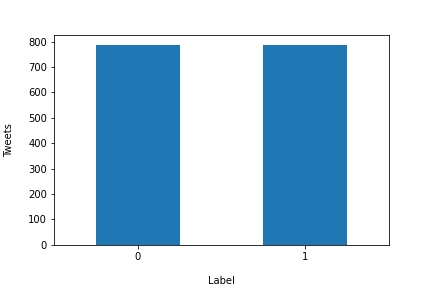
\includegraphics[width= 0.8\textwidth]{images/dataset/training set.png} 
    \caption{Labeled tweets of the training set} 
    \label{classes}
\end{figure}





\subsection{Preprocessing}

After the tweets have been comprehended and correctly labeled some other useless information can be removed. These steps are:

\begin{itemize}
\item  removing \textbf{punctuation}: markers, quotes, brackets, special characters;
\item \textbf{text reformat}: removing of multiple dots and multiple last letters, lower case of the text;
\item \textbf{emojis} removal;
\end{itemize}
At the end of this phase, an Elaboration one follows. The aim of this step is to transform a set of strings (the preprocessed tweets), in a set of numeric vectors ready to be elaborated by the Classification module. 
These are the steps performed in order to obtain the aimed result: 
\begin{itemize}
\item \textbf{tokenization}: consists of brake the raw text into chunks, denominated tokens. Each token corresponds to a single word. At the end of this step, have been obtained a sequence of words for each tweet;
\item \textbf{stop-word filtering}: removing of stop-words like articles or prepositions that have no significance for the project analysis purpose;
\item \textbf{stemming}: is the process of reducing words to their root form;
\item remove \textbf{miningless words}: all the words with number of characters less or equal than two have been discarded;
\item remove \textbf{only-digit features}: removal of features composed only by digits
\end{itemize}



\begin{figure}[H]
    \centering
    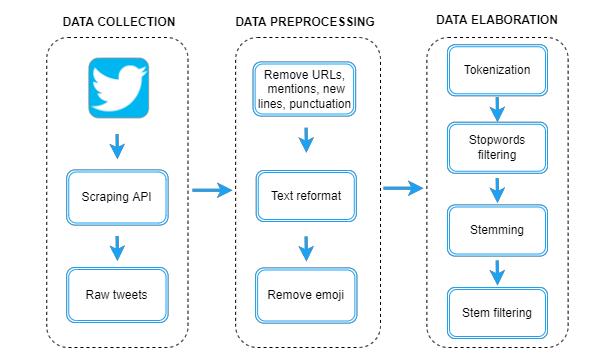
\includegraphics[width=0.8\textwidth]{images/dataset/preprocessing.png} 
    \caption{Data fetching and preprocessing} 
    \label{fig:preprocessing}
\end{figure}





\subsection{Feature extraction and selection}
The training set has been built starting from the preprocessed tweets, characterized by 788 tweets classified as 'body shaming' and 788 other tweets 'non-body shaming'.
Using the \emph{sklearn.feature\_extraction} library of Python every model has been integrated as the last step of pipeline composed by the following steps:

\begin{itemize}
\item \textbf{vectorization} using CountVectorizer() with ngram = 1 the collection of tweets is converted to a matrix of token counts;
\item  \textbf{Tf-Idf}: This weight is a statistical measure used to evaluate how important a word (stem) is to a document (tweet) in a collection or corpus. The importance increases proportionally to the number of times a word appears in the document but is offset by the frequency of the word in the corpus (data-set);
\item \textbf{feature selection} using SelectPercentile() with \emph{percentage} parameter equal to 75, a number of features equal to about 3500, with respect to the initial 4669, has been obtained. \end{itemize}

\noindent
For the feature selection phase, different values of percentage have been compared.


\begin{figure}[H]
\centering
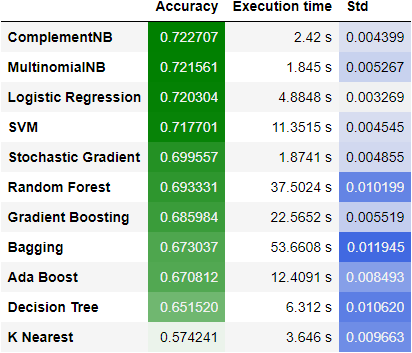
\includegraphics[width=.47\textwidth]{images/features/cross_val_result_75.png}\hfil
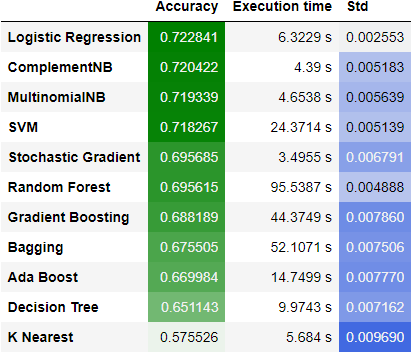
\includegraphics[width=.47\textwidth]{images/features/cross_val_result_85.png}

\caption{Percentage of feature selection compared: 75\%, 85\%}\label{fig:75-85}
\end{figure}

\noindent
As shown in the table \ref{fig:75-85}, regardless of the percentage of selected features, the 4 classifiers that perform best are: \emph{Logistic Regression}, \emph{SVM}, \emph{ComplementNB} and \emph{MultinomialNB}. These algorithms have the best accuracy and lowest standard deviation. Considering the execution times all perform well except for SVM that is the slowest.

Changing the feature percentage the accuracy does not change a lot therefore, focusing on \emph{Logistic Regression}, \emph{ComplementNB} and \emph{MultinomialNB}, the standard deviation and the execution times are lower with a value of 75\% that allows to lighten the computation.
Moreover, in this scenario the best 4 classifiers will be compared with some metrics.
\section{Model training and testing}

Starting from the features selected in the previous steps, a model prediction phase followed. This has been done, first of all, using the k-fold cross validation technique. It has been applied with a number of folders equal to 10 and repeated more than one time as suggested in \cite{traffic}. In this work the validation was repeated for a number of iterations equal to 10.

\begin{figure}[H]
\centering
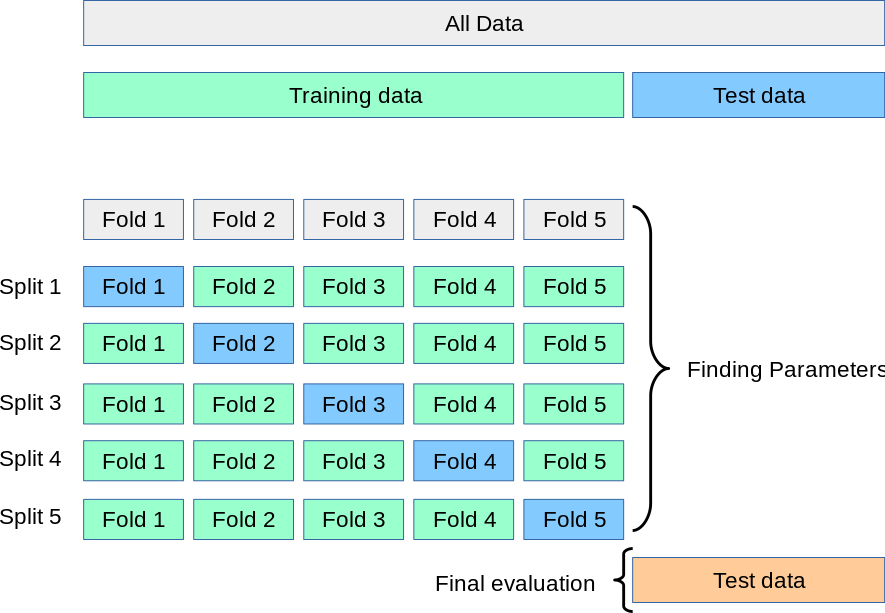
\includegraphics[width=10cm]{images/training/cross_validation.png}
\caption{Cross-validation example}
\label{cross-validation}
\end{figure}

\noindent
The output, composed by ten elements, each one representing the mean of the accuracy of one 10-fold iteration, has been used in order to perform the statistical test.

\subsection{Model selection}

Some classifiers have been discarded after comparing some parameters shown in \ref{fig:75-85}: \emph{K Nearest}, \emph{Decision Tree} and \emph{Stochastic Gradient} because of their low accuracy compared to the others and \emph{Random Forest}, \emph{Gradient Boosting}, \emph{Bagging} and \emph{Ada Boost} because of their high execution time.

\noindent
The remaining classifiers have been compared in terms of accuracy (more than 70\%), precision, recall and f1-score.

\vspace{5mm}

\setlength{\tabcolsep}{5pt}
\renewcommand\arraystretch{1.5}
\begin{table}[H]
\centering
\begin{tabular}{lc cc c cc c cc}
\hline
\multirow{2}*{Classifier} & \multirow{2}*{Accuracy (\%)} & \multicolumn{2}{c}{Precision (\%)} && \multicolumn{2}{c}{Recall (\%)} && \multicolumn{2}{c}{F1-score (\%)}\\
\cline{3-4} \cline{6-7} \cline{9-10}
\multicolumn{1}{c}{} && 0 & 1 && 0 & 1 && 0 & 1 \\
\hline
Logistic Regression & 72.52 & 71.00 & 74.28 && 76.14 & 68.90 && 73.48 & 71.49 \\
SVM                 & 71.76 & 70.63 & 73.02 && 74.49 & 69.03 && 72.51 & 70.97 \\
\hline
\end{tabular}
\caption{Report comparison \emph{Logistic Regression} and \emph{SVM}}
\label{training-LR-SVM}
\end{table}

\noindent
\emph{Logistic Regression} performs better than \emph{SVM} considering all the metrics (Table  \ref{training-LR-SVM}). 

\setlength{\tabcolsep}{5pt}
\renewcommand\arraystretch{1.5}
\begin{table}[H]
\centering
\begin{tabular}{lc cc c cc c cc}
\hline
\multirow{2}*{Classifier} & \multirow{2}*{Accuracy (\%)} & \multicolumn{2}{c}{Precision (\%)} && \multicolumn{2}{c}{Recall (\%)} && \multicolumn{2}{c}{F1-score (\%)}\\
\cline{3-4} \cline{6-7} \cline{9-10}
\multicolumn{1}{c}{} && 0 & 1 && 0 & 1 && 0 & 1 \\
\hline
ComplementNB        & 73.03 & 72.21 & 73.91 && 74.87 & 71.19 && 73.52 & 72.52 \\
MultinomialNB       & 72.39 & 71.87 & 72.95 && 73.60 & 71.19 && 72.72 & 72.06 \\
\hline
\end{tabular}
\caption{Report comparison of \emph{ComplementNB} and \emph{MultinomialNB}}
\label{training-CNB-MNB}
\end{table}

\noindent
Comparing the Naive Bayes classifiers, \emph{ComplementNB} is preferred (Table  \ref{training-CNB-MNB}).

\subsection{Paired t-test}

The paired t-test has been performed to compare the four classifiers two-by-two to establish if their performances are statistically different or not starting from a null hypothesis saying that they are the same or, in other words, that the difference in mean error rate between the two is zero. If we can reject this hypothesis, then we can conclude that the difference between the two models is statistically significant, so can be selected the model with the lower error rate (higher accuracy) \cite{book}.

The scores obtained are k=10 and the degree of freedom considered are k-1. By computing the t-statistic value and using a significance level \begin{math}sig = 0.05\end{math} and a confidence limit of \begin{math}z = 0.025\end{math} (that is half of sig) some considerations can be done comparing t with a value j obtained from the t-distribution table: if \begin{math}t > j\end{math} or \begin{math}t < -j\end{math} the null hypothesis is rejected and there is statistically significant difference between the two models, otherwise the hypothesis cannot be rejected and this means that any difference between them is attributed by chance.

\vspace{5mm}

\noindent
Figure \ref{t-test} shows the result of the paired t-test executed on the 4 different classifiers.


\begin{figure}[H]
\centering
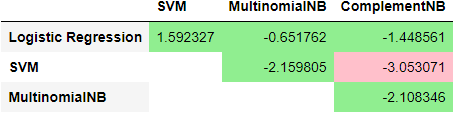
\includegraphics[width=10cm]{images/training/t_test_result.png}
\caption{Student T-test result}
\label{t-test}

\begin{figure}[H]
\end{figure}
\centering
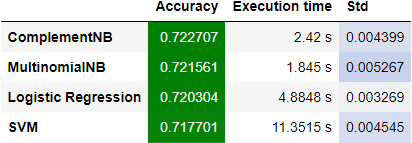
\includegraphics[width=10cm]{images/training/best_cv.png}
\caption{Performances compared}
\end{figure}

\noindent
The pink cells indicate the comparable classifiers while the green ones are related to the non-comparable ones. Reading Table \ref{t-test} row by row some considerations can be done:
\begin{itemize}
    \item The difference between \emph{SVM} and \emph{ComplementNB} is statistically significant, but \emph{SVM} has a worse accuracy with respect to \emph{ComplementNB}, so ComplementNB have been chosen;
\end{itemize}

\noindent
At the end, \emph{ComplementNB}, \emph{MultinomialNB} and \emph{Logistic Regression} models are taken into consideration and used for the test phase. 

\begin{figure}[h]
\centering
\begin{minipage}[c]{0.48\textwidth}
\centering
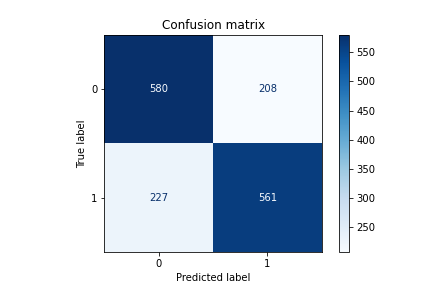
\includegraphics[width=8cm]{images/training/MultinomialNB-confusion_matrix.png}
\caption{MultinomialNB}
\end{minipage}
\begin{minipage}[c]{0.48\textwidth}
\centering
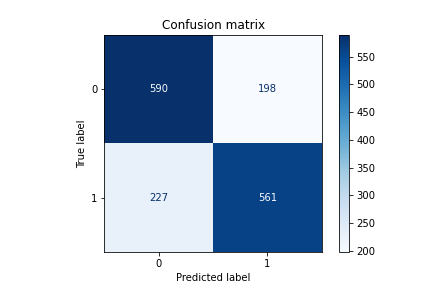
\includegraphics[width=8cm]{images/training/ComplementNB-confusion_matrix.png}
\caption{ComplementNB}
\end{minipage}
\end{figure}


\begin{figure}[H]
\centering
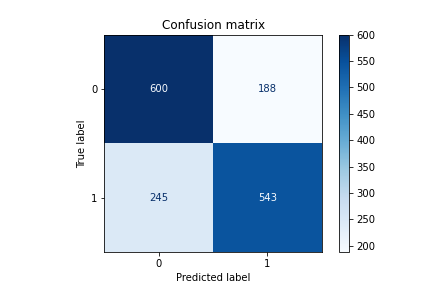
\includegraphics[width=8cm]{images/training/Logistic Regression-confusion_matrix.png}
\caption{LogisticRegression}
\end{figure}


\subsection{Model testing}

After the model building phase, the test phase has been performed. In order to test the performance of the models, 176 tweets from February were randomly and manually labeled, corresponding to a proportion 90:10 with respect to the training set. Testing the models built in the precedent phase, the results shown in Table \ref{table:test} below have been obtained. 
\vspace{5mm}
\begin{table}[H]
\centering
\setlength{\tabcolsep}{5pt}
\renewcommand\arraystretch{1.5}
\begin{tabular}{lc cc c cc c cc}
\hline
\multirow{2}*{Classifier} & \multirow{2}*{Accuracy (\%)} & \multicolumn{2}{c}{Precision (\%)} && \multicolumn{2}{c}{Recall (\%)} && \multicolumn{2}{c}{F1-score (\%)}\\
\cline{3-4} \cline{6-7} \cline{9-10}
\multicolumn{1}{c}{} && 0 & 1 && 0 & 1 && 0 & 1 \\
\hline
ComplementNB                 & 73.29 & 71.13 & 75.94 && 78.40 & 68.18 && 74.59 & 71.85 \\
Logistic Regression         & 71.59 & 68.26 & 76.38 && 80.68 & 62.50 && 73.95 & 68.75 \\
MultinomialNB                 & 73.29 & 71.13 & 75.94 && 78.40 & 68.18 && 74.59 & 71.85 \\
\hline
\end{tabular}
\caption{Report comparison of Logistic Regression and ComplementNB}
\label{table:test}
\end{table}

\noindent
As shown in Table \ref{table:test}, ComplementNB and MultinomialNB performs a little bit better than the training set instead of the Logistic Regression which performs a little worse. ComplementNB and MultinomialNB have the same performance in this phase but ComplementNB have been chosen because of its better performance in the training set phase. 
\section{Online monitoring}

The model just built is now ready to be used to classify the upcoming tweets. Predictive modeling consists in learning a model from historical data and using the model to make predictions on new data where the answer is unknown. For this reason, it is possible that a model built on past data can not be suitable for the analysis of subsequent data.

It is well known from the literature that classification models for analyzing streams of data suffer from \textbf{concept drift}. In predictive analytics and machine learning, the concept drift means that the statistical properties of the target variable, which the model is trying to predict, change over time in unexpected ways. This causes problems because predictions may become less accurate as time goes on.

For what concern text mining this problem occurs because people may change the way they express their ideas on social medias according to real world events. The consequence is that the volume of the data collected can be different and the features may change. 
If these changes are able to be detected, it may be possible to update the learned model to avoid performance loss. 

\subsection{Identifying peaks}

In order to understand if the ComplementNB model, built in the previous phases, suffers from concept drift, some {peaks},  probably corresponding to some events verified immediately before, have been identified from the overall distribution of the collected tweets  in the period following the test (Figure \ref{online-monitoring}). 

The goal is to analyze the behaviour of the built model during the days associated with the occur of some  events. Indeed, during these days, a change of the terminology used is expected and, for this reason, the corresponding tweets are particularly useful to highlight the concept drift. 
The objective of this analysis is to adapt the vocabulary used by the model in order to find a way to alleviate the concept drift.

The days highlighted in the diagram in Figure \ref{online-monitoring} correspond to the peaks chosen for the experiments conducted on the concept drift. \textbf{80 tweets} were randomly selected from every peak, except for the last peak for which were selected only \textbf{60 tweets} because the number of tweets decreases. Moreover, since no relevant peaks were found in May, 80 tweets were randomly taken from the entire month.
The peak corresponding to the 1st of March has been discarded because too close to the test set: in a more central date with respect to the month, as 2022-03-10, the effects of concept drift may be more evident.

\begin{figure}[H]
    \centering
    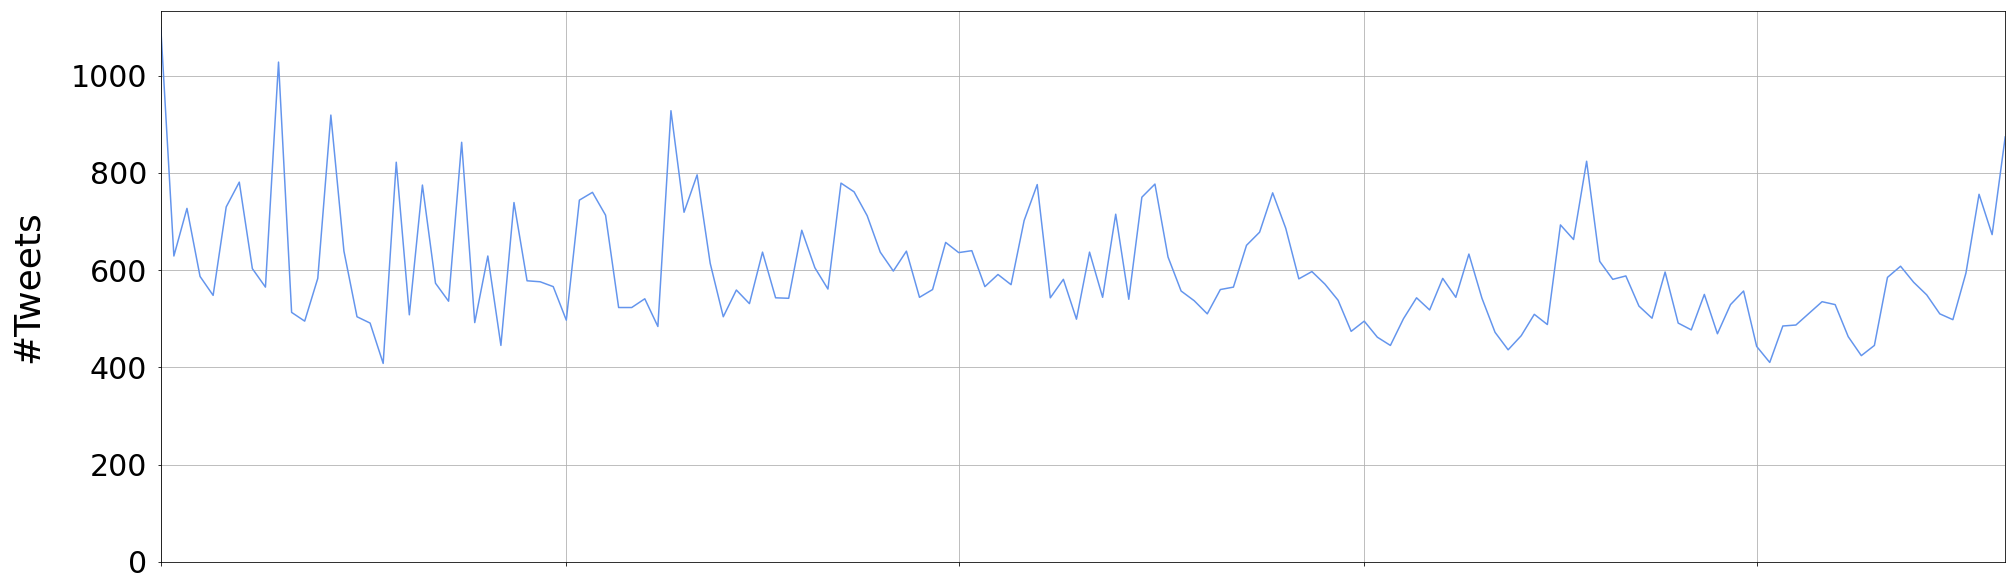
\includegraphics[width=1\textwidth]{images/monitoring/monitoring_lineplot_noX.png}
    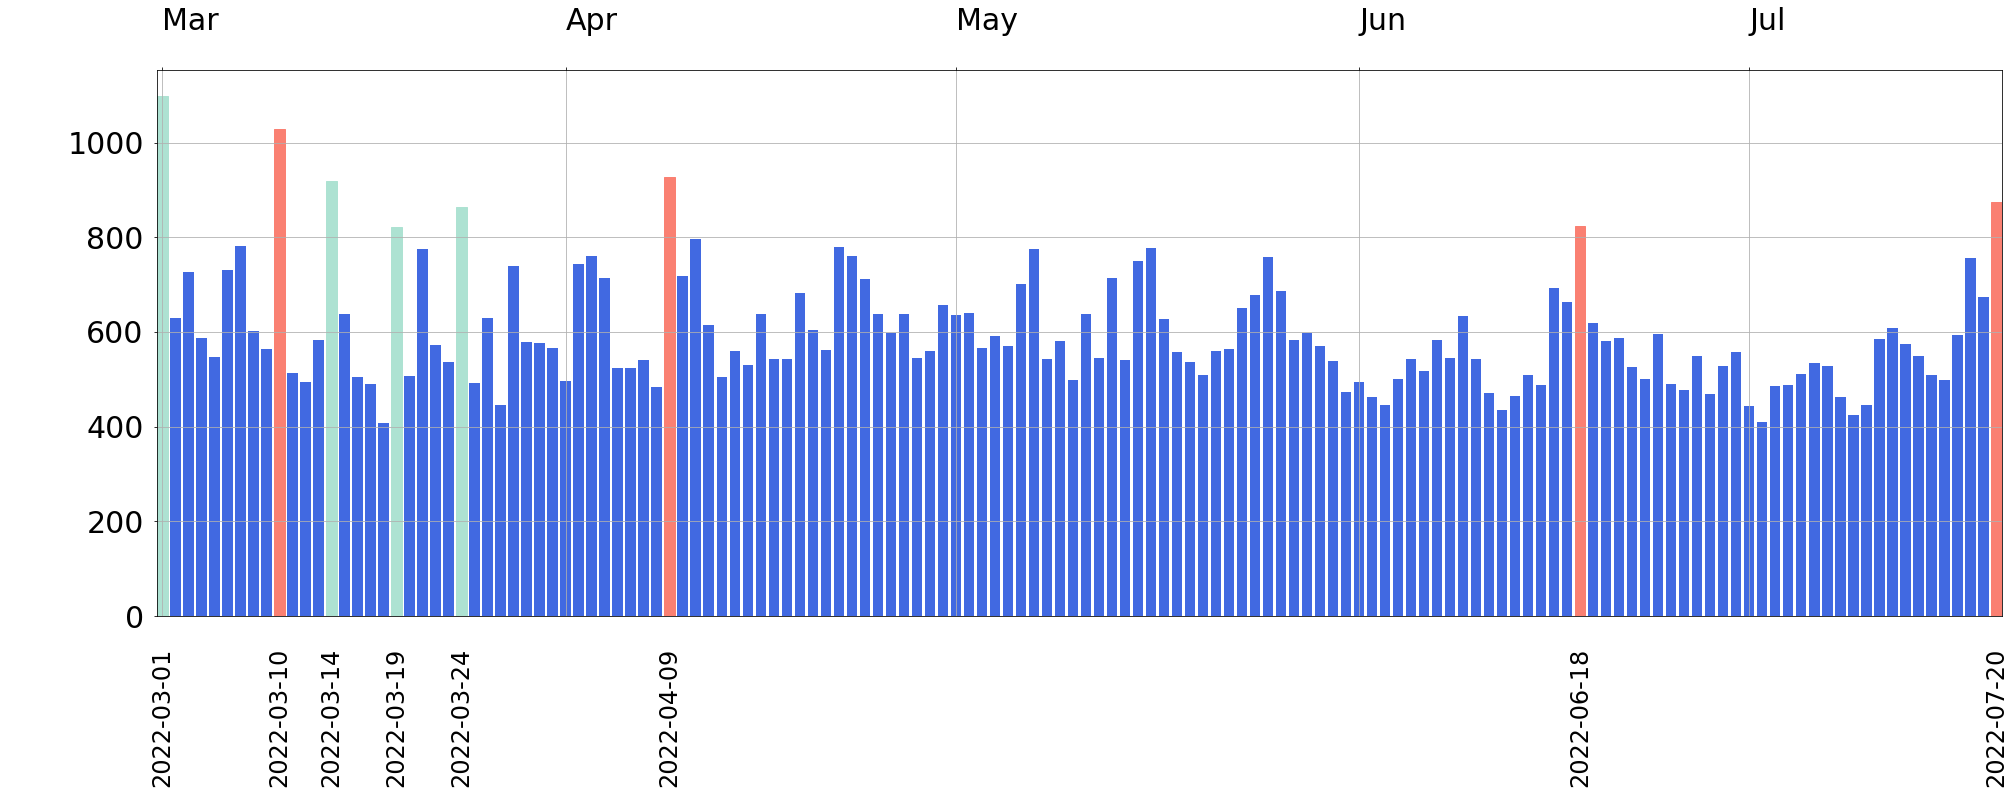
\includegraphics[width=1\textwidth]{images/monitoring/monitoring_barplot_peaks.png}
    \caption{Tweets distribution from 1st March, 2022 to 30th June, 2022} 
    \label{online-monitoring}
\end{figure}


\noindent
Table \ref{table:peaks} describes how many tweets have been collected in every temporal period and the hypothetical events that may have caused an increase in the volume of tweets posted.
\vspace{5mm}

\begin{table}[H]
\centering
\setlength{\tabcolsep}{5pt}
\renewcommand\arraystretch{1.5}
\begin{tabular}{cllp{6cm}r}
\hline
Name & Peak/Period & Date/Month & Event & Tweets \\
\hline
Period1 & Peak 1 & 2022-03-10 & Tv program GF semifinal & 1028 \\
Period2 & Peak 2 & 2022-04-09 & Episode of the tv program Amici with Sangiovanni as host  & 928  \\
Period3 &  May   & 2022-05    &    & 18959\\
Period4 & Peak 4 & 2022-06-18 & Vanessa Incontrada host of Gigi D'alessio's tv show & 824  \\
Period5 & Peak 5 & 2022-07-20 & Government crisis & 874\\
\hline
\end{tabular}
\caption{Peak/period details}
\label{table:peaks}
\end{table}

\vspace{5mm}
\vspace{5mm}
\subsection{Testing concept drift}

As suggested in \cite{greenpass} the 3 different types of concept drift that can be examinated are:

\begin{itemize}
    \item \textbf{static}, in which the model is always the same and it is tested using new tweets;
    \item \textbf{sliding window}, in which the model is retrained adding n new tweets and removing the older n ones;
    \item \textbf{incremental}, that retrains the model adding new labeled tweets also considering all the previous ones.
\end{itemize}

\noindent
For each event, except for the last one where only 60 tweets were taken, 80 tweets were randomly selected, manually labeled and used as test set for the \textbf{static model} to verify if the concept drift can really be a problem for this work.  

\vspace{5mm}
\begin{table}[H]
\centering
\setlength{\tabcolsep}{5pt}
\renewcommand\arraystretch{1.5}
\begin{tabular}{llc cc c cc c cc}
\hline
\multirow{2}*{Name} & \multirow{2}*{Peak} & \multirow{2}*{Accuracy (\%)} & \multicolumn{2}{c}{Precision (\%)} && \multicolumn{2}{c}{Recall (\%)} && \multicolumn{2}{c}{F1-score (\%)}\\
\cline{4-5} \cline{7-8} \cline{10-11}
\multicolumn{1}{c}{} &&& 0 & 1 && 0 & 1 && 0 & 1 \\
\hline
Period1 & Peak 1 & 73.75 & 74.35 & 73.17 && 72.50 & 75.00 && 73.41 & 74.07 \\
Period2 & Peak 2 & 72.50 & 70.45 & 75.00 && 77.50 & 67.50 && 73.80 & 71.05 \\
Period3 &  May   & 73.75 & 72.09 & 75.67 && 77.50 & 70.00 && 74.69 & 72.72 \\
Period4 & Peak 4 & 66.25 & 64.44 & 68.57 && 72.50 & 60.00 && 68.23 & 64.00 \\
Period5 & Peak 5 & 60.00 & 60.71 & 59.37 && 56.66 & 63.33 && 58.62 & 61.29 \\
\hline
\end{tabular}
\caption{Static model}
\label{table:static}
\end{table}
\noindent
For incremental and sliding approach, the training set have been updated basing on the behaviour of the different approaches. 

The \textbf{sliding approach} provides a new model for each new chunk of tweets, discarding the oldest and adding the newest, following the window dimension. The window dimension chosen was of 80 tweets (60 for July). For each peak, the new 80 (60) labeled tweets were inserted into the training set and the same number of the oldest tweets were removed. In this way, the number of tweets considered for the training set was always the same. The model is retrained each time considering the new tweets and the number of features changes during the various peaks. 


\vspace{5mm}
\begin{table}[H]
\centering
\setlength{\tabcolsep}{5pt}
\renewcommand\arraystretch{1.5}
\begin{tabular}{llc cc c cc c cc}
\hline
\multirow{2}*{Name} & \multirow{2}*{Peak} & \multirow{2}*{Accuracy (\%)} & \multicolumn{2}{c}{Precision (\%)} && \multicolumn{2}{c}{Recall (\%)} && \multicolumn{2}{c}{F1-score (\%)}\\
\cline{4-5} \cline{7-8} \cline{10-11}
\multicolumn{1}{c}{} &&& 0 & 1 && 0 & 1 && 0 & 1 \\
\hline
Period1 & Peak 1 & 73.75 & 72.09 & 75.67 && 77.50 & 70.00 && 74.69 & 72.72 \\
Period2 & Peak 2 & 76.25 & 70.58 & 86.20 && 90.00 & 62.50 && 79.12 & 72.46 \\
Period3 & May    & 71.25 & 68.08 & 75.75 && 80.00 & 62.50 && 73.56 & 68.49 \\
Period4 & Peak 4 & 71.25 & 69.76 & 72.97 && 75.00 & 67.50 && 72.28 & 70.12 \\
Period5 & Peak 5 & 63.33 & 64.28 & 62.50 && 60.00 & 66.66 && 62.06 & 64.51 \\
\hline
\end{tabular}
\caption{Sliding model}
\label{table:sliding}
\end{table}

\noindent
The \textbf{incremental approach} foresees a new retrain of the model each time basing on a training set gradually incremented with the previous examples. The approach adopted is not purely incremental but it is an approach that re-evaluates the model at every new peak. At each peak the training set have been incremented using the tweets of the previous peaks. In this way, at the end, the dimension of the training set goes from 1576 to 2132. With this approach, as consequence of the increasing of the training set dimension, the number of features increases too. 

\vspace{5mm}
\begin{table}[H]
\centering
\setlength{\tabcolsep}{5pt}
\renewcommand\arraystretch{1.5}
\begin{tabular}{llc cc c cc c cc}
\hline
\multirow{2}*{Name} & \multirow{2}*{Peak} & \multirow{2}*{Accuracy (\%)} & \multicolumn{2}{c}{Precision (\%)} && \multicolumn{2}{c}{Recall (\%)} && \multicolumn{2}{c}{F1-score (\%)}\\
\cline{4-5} \cline{7-8} \cline{10-11}
\multicolumn{1}{c}{} &&& 0 & 1 && 0 & 1 && 0 & 1 \\
\hline
Period1 & Peak 1 & 71.25 & 68.88 & 74.28 && 77.50 & 65.00 && 74.94 & 69.33 \\
Period2 & Peak 2 & 73.75 & 69.38 & 80.64 && 85.00 & 62.50 && 76.40 & 70.42 \\
Period3 & May    & 72.50 & 70.45 & 75.00 && 77.50 & 67.50 && 73.80 & 71.05 \\
Period4 & Peak 4 & 70.00 & 69.04 & 71.05 && 72.50 & 67.50 && 70.73 & 69.23 \\
Period5 & Peak 5 & 66.66 & 65.62 & 67.85 && 70.00 & 63.33 && 67.74 & 65.51 \\
\hline
\end{tabular}
\caption{Incremental model}
\label{table:incrementa}
\end{table}

\noindent
As it is possible to observe in the (Figure \ref{online-monitoring-accuracy}), the more time goes on the more the model designed with the static approach does not perform well. The other two, indeed, perform better during the time. Moreover, it is possible to observe that the static model has decreasing performances during the peaks but performs not so bad in May in which there is no event. The sliding, however, performs better than the incremental during all the peaks except for May and the last peak. 

\begin{figure}[H]
    \centering
    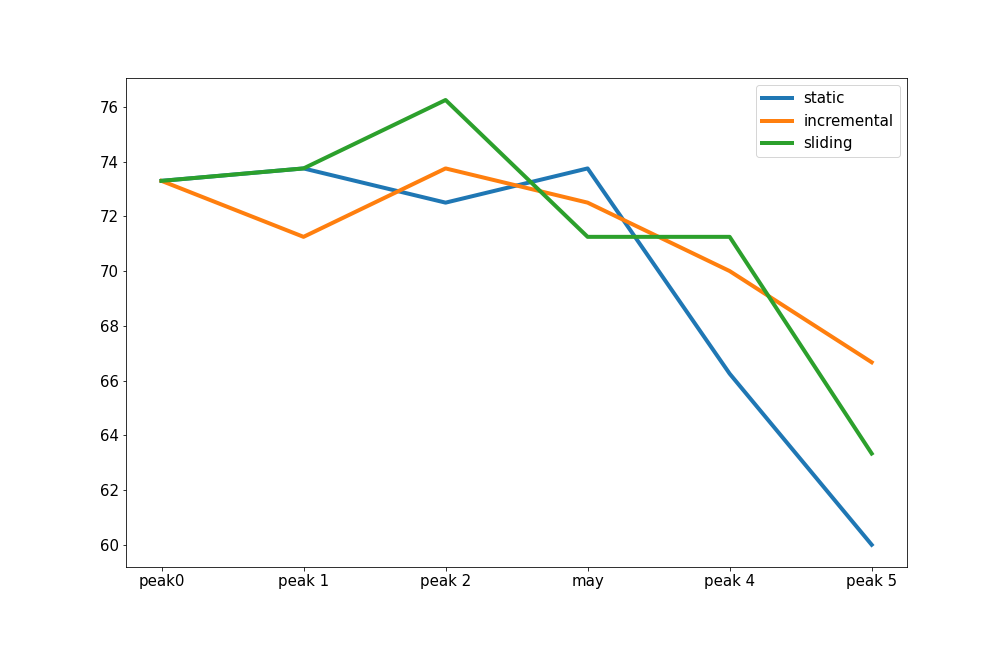
\includegraphics[width= 1\textwidth]{images/monitoring/accuracy_for_model.png}
    \caption{Accuracy for the three approaches} 
    \label{online-monitoring-accuracy}
\end{figure}

\noindent
The sliding approach results the one with the best performance except for the last peak. At the same time, the number of features of the incremental model increases quickly. On the contrary, the number of features using the sliding approach are always very low. 

\begin{figure}[H]
    \centering
    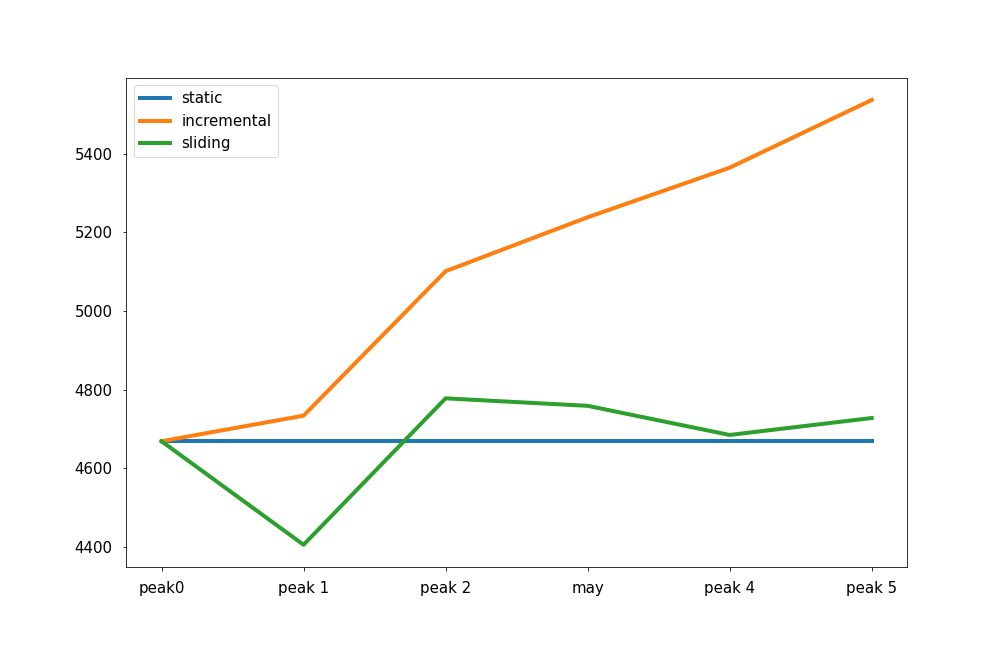
\includegraphics[width= 1\textwidth]{images/monitoring/features_for_model.png}
    \caption{Number of features for each approach} 
    \label{online-monitoring-features}
\end{figure}

\noindent
At the end, the sliding approach have been chosen. Indeed, the performance with this approach are mostly the best in the peaks and at the same time the number of features is low. However, in the last peak its performances decrease quickly and, for this reason, there is the possibility that in a long period the incremental approach will be more suitable than the sliding. The decrease in performance could be due to the fact that all the precedent peaks concern television programs events whereas, the last one, concerns a political event. It is possible that, considering an additional time period, the incremental approach will reveal to be the best choice.  


\section{Application}

The application provides a body-shaming detection service. 

\subsection{Use cases}

This application provides a service of real time body shaming detection. It scrapes tweets from Twitter and, using the model built in the precedent steps, evaluates which user is doing body shaming in the time period selected by the user. 
The application has been thought as a simple tool that a Twitter moderator can use to detect a shamer user in order to block him. Indeed, automatically,  the tweets scraped are saved into a csv file and, if a user has been found more than a specific number of times, he/she is inserted into a blacklist. 

\begin{figure}[H]
    \centering
    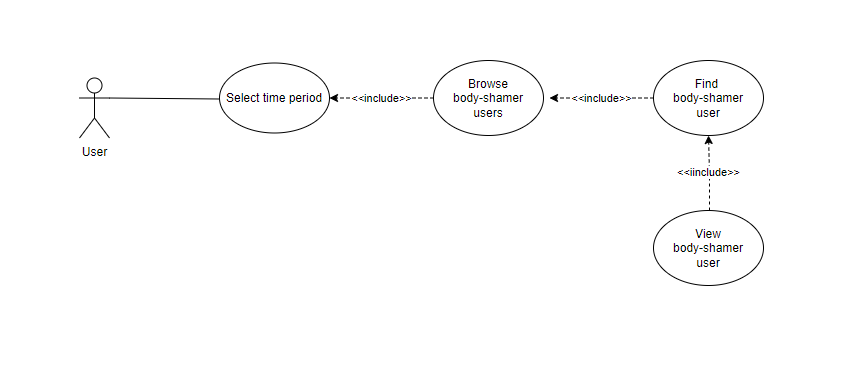
\includegraphics[width= 1.05\textwidth]{images/application/usecases.PNG}
    \caption{Application use cases} 
    \label{application-use-cases}
\end{figure}

\subsection{User Manual}
\begin{figure}[H]
    \centering
    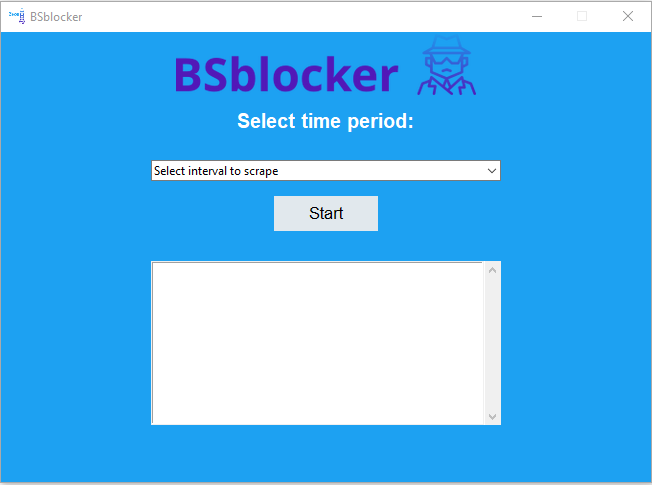
\includegraphics[width= 0.8\textwidth]{images/application/homepage.png}
    \caption{Application home page} 
    \label{application-home}
\end{figure}
\noindent
The user can select a time period in which the application will scan the tweets in order to find out the users that have been done body-shaming. After selecting the period, it is only necessary to press the 'Start' button to let the process start. 
When the detection ends, the name of the users that have done body-shaming appears in the scroll bar below. 

\begin{figure}[H]
    \centering
    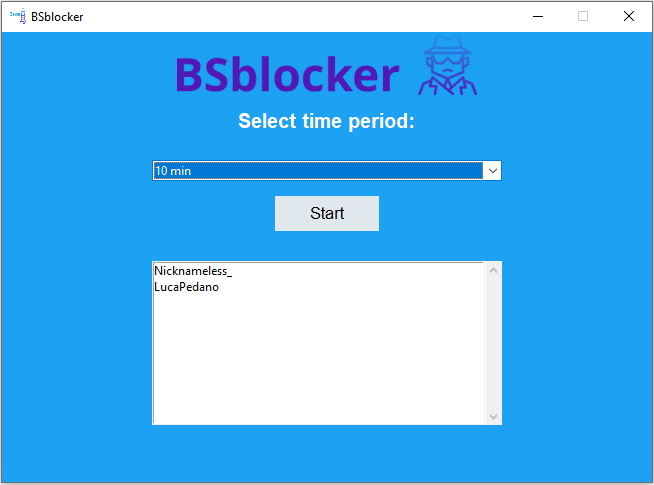
\includegraphics[width= 0.8\textwidth]{images/application/scrape.png}
    \caption{Detection result} 
    \label{use-cases}
\end{figure}

\noindent
When one of the shown users has been detected more than 5 times, it is colored in red.


\begin{figure}[H]
    \centering
    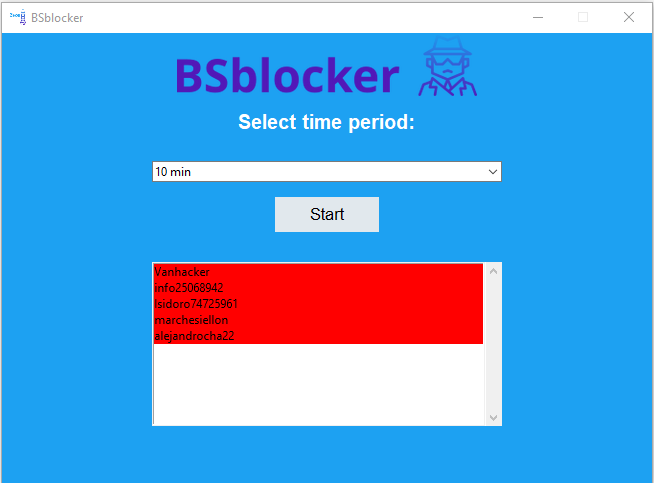
\includegraphics[width= 0.8\textwidth]{images/application/blacklist.PNG}
    \caption{Users in blacklist} 
    \label{application-blacklist}
\end{figure}






\subsection{Conclusion}

In conclusion, the work described in this documentation has provided satisfying results and a valid model for the body shaming detection. 
Moreover, an application for this purpose, for the real time body shaming detection, has been developed in order to let a user, more specifically a twitter moderator, detect users doing body shaming. 

Surely, the model could be updated and the best approach to cope with concept drift may be re-evaluated, in order to maintain good performances. 

\vspace{5mm}
\vspace{5mm}
\vspace{5mm}

\noindent
To visit the repository click \href{https://github.com/martimarino/Body-shaming-detection.git}{here}.

\cleardoublepage
\phantomsection
\addcontentsline{toc}{section}{References}

\bibliographystyle{plain}
\bibliography{chapters/bibliography.bib}

\end{document}
% -----------------------------------------------------------------